\chapter{Classification Results}
\label{sec:results}

\ifpdf
    \graphicspath{{7_results/figures/PNG/}{7_results/figures/PDF/}{7_results/figures/}}
\else
    \graphicspath{{7_results/figures/EPS/}{7_results/figures/}}
\fi

Accuracy score is typically used to identify optimal models, however as a metric it is often not interpretable and discriminative \cite{hossin2015review}. Moreover, an accuracy score is almost always biased towards the majority class. The goal was to ensure that timeslices with neutrinos did not get mislabelled as noise. Therefore, \textit{recall} was the most significant metric for the classification task.
Based on the highly imbalanced nature of the dataset and the physics goal, a few other metrics were also required \cite{scikit-learn}. This chapter establishes the relevant metrics selected for classification and discusses the results obtained through plots and summaries. 

\textbf{Precision} measures the percentage of results that are relevant. It is the ability of the classifier to not label a negative sample as positive \cite{scikit-learn}. Precision is given by the number of true positives (${T}_p$) over the number of true positives (${T}_p$) plus the number of false positives (${F}_p$):
    \[
        P = \frac{{T}_p}{{T}_p + {F}_p}
    \]
    
\textbf{Recall} refers to the percentage of total relevant results correctly classified, and is the ability of the classifier to find all positive samples \cite{scikit-learn}. It is given by the number of true positives (${T}_p$) over the number of true positives (${T}_p$)  plus the number of false negatives (${F}_n$):
    \[
        R = \frac{{T}_p}{{T}_p + {F}_n}
    \]

\textbf{F1 Score} is a weighted harmonic mean of the precision and recall \cite{scikit-learn}. It is given by:
    \[
        F1 = 2 \times \frac{P \times R}{P + R}
    \]

\textbf{Receiver Operating Characteristic (ROC) Curves} depict the trade-off between true positive rate and false positive rate for different probability thresholds \cite{scikit-learn}.
 
\textbf{Precision-Recall (PR) Curve} shows the trade-off between precision and recall for different thresholds \cite{scikit-learn}. A high area under the curve represents both high recall and high precision. 

\textbf{Confusion Matrix} visualises the number of true positives, false positives, true negatives and false negatives \cite{jaffery2009measuring} . 

Each of the three datasets - (\texttt{x, y, time}),  (\texttt{x, z, time}), and (\texttt{y, z, time}) were trained using the same PointNet model parameters (Table \ref{tab:model_parameters}), and their results combined using ensemble techniques. Table \ref{tab:results} shows the final classification accuracy scores for each of the three datasets and the results after applying two majority voting ensemble methods. 

\begin{table} [ht!]
    \centering
    \begin{tabular}{l c}
    \hline
        \texttt{x, y, time} & \textbf{95\% } (loss = 0.003)\\
        \texttt{x, z, time} & \textbf{90\%} (loss = 0.006)\\
        \texttt{y, z, time} & \textbf{99\%} (loss = 0.005)\\
        Ensemble 1: Hard Voting & \textbf{97\%}\\
        Ensemble 2: Soft Voting & \textbf{90\%}\\
    \hline
    \end{tabular}
    \caption{Accuracy Scores}
    \label{tab:results}
\end{table}

A classification report was generated for each dataset and the two ensembles to obtain detailed performance report on precision, recall and F1 Scores. ROC Curves and PR Curves were both plotted to compare against each other. This is because ROC curves are more appropriate for balanced classes and PR curves are better suited for imbalanced datasets. Keeping in mind the physics goal, analysis was more focused on the model's performance in (mis)classifying event timeslices (\texttt{class\_1}). 

\section{Dataset 1: \texttt{x, y, time}}

The \texttt{x, y, time} model reported a 95\% accuracy. Classification report in Table \ref{tab:xyt_classification_report} shows that the model did not mislabel any noise (\texttt{class\_0}) as event \texttt{class\_1} timeslices. Further, \textbf{90\%} of the total relevant results were correctly classified as \texttt{class\_1}. Support indicates that 40 test cases were used for each class.

\begin{table} [ht!]
    \centering
    \begin{tabular}{l c c c c}
    \hline
    \multicolumn{5}{c}{\texttt{x, y, time}} \\
    \hline
                     & precision  & recall& F1-score & support \\
        \texttt{class\_0} & 0.91  &  1.00    & 0.95 & 40\\
        \texttt{class\_1} & 1.00  &  0.90    & 0.95 & 40\\
    \hline
    \end{tabular}
    \caption{\texttt{x, y, time}: Classification Report for \texttt{class\_0} and \texttt{class\_1}}
    \label{tab:xyt_classification_report}
\end{table}

Figure \ref{fig:xyt_results} shows the relevant plots  of metrics for the dataset. The ROC curves are towards the top left of the graph and indicate a desirable, high true positive rate against the baseline performance plotted on the diagonal. Complementing the ROC, the Precision-Recall (PR) curves show a high area under the curve, indicating high precision and recall. Precision was mostly stable for increasing recall, but it fell dramatically for \texttt{class\_1} after 85\% recall. The confusion matrix shows that 4 of the 40 timeslices with event hits were incorrectly labelled as noise, but none of the noise timeslices were incorrectly labelled.
 
\begin{figure}[ht!]
    \centering
    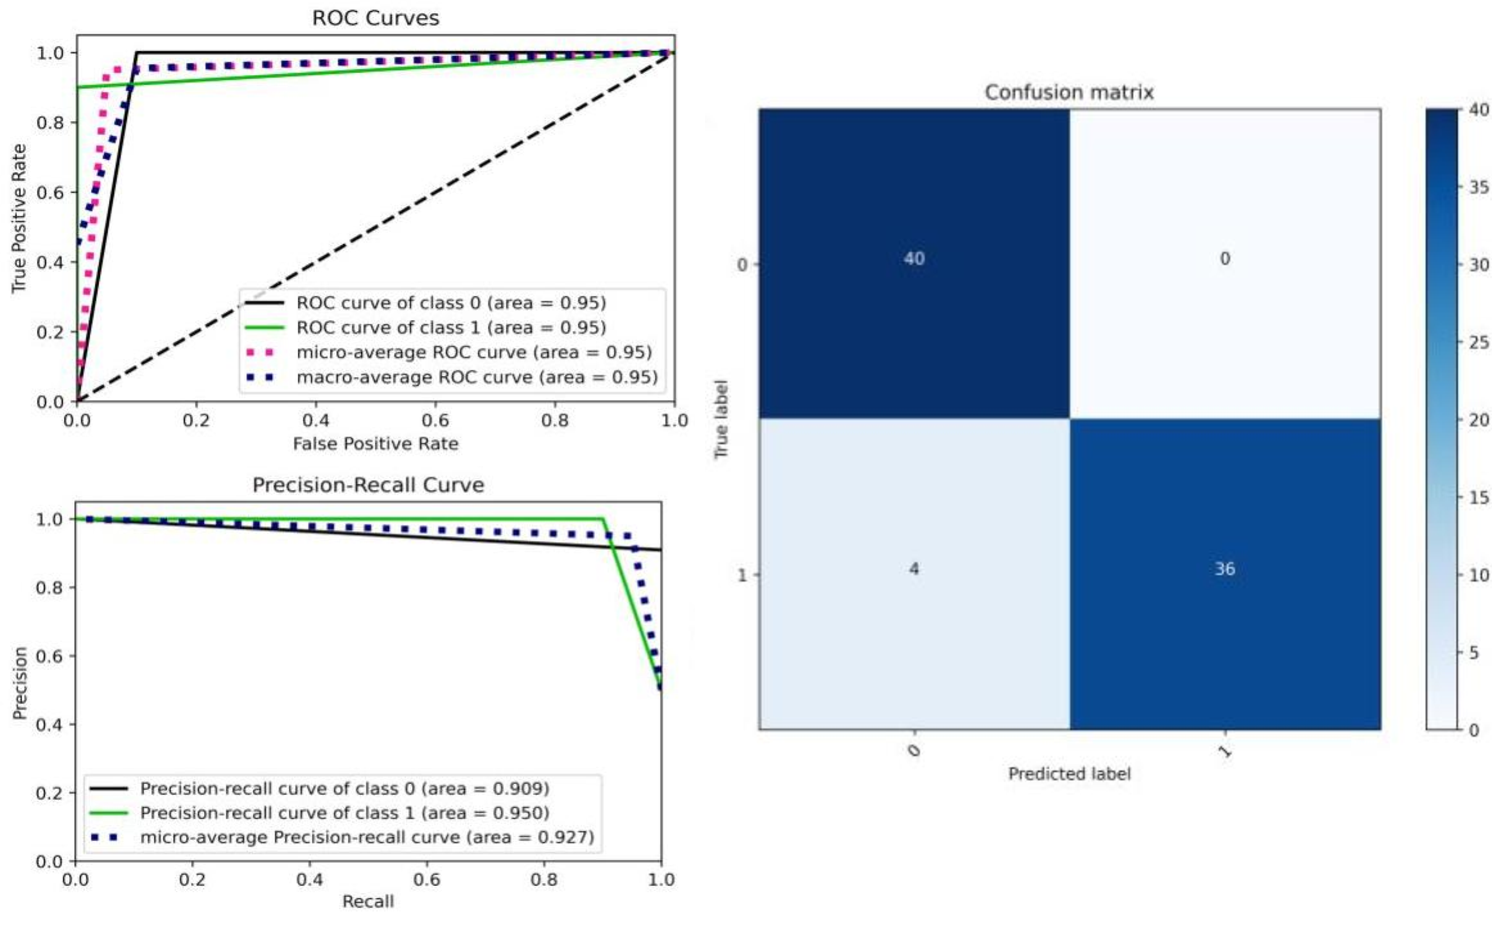
\includegraphics[width=\textwidth,keepaspectratio]{xyt.pdf}
    \caption{\texttt{x, y, time}: Classification Plots}
    \label{fig:xyt_results}
\end{figure}

\section{Dataset 2: \texttt{x, z, time}}
\begin{table} [ht!]
    \centering
    \begin{tabular}{l c c c c}
    \hline
    \multicolumn{5}{c}{\texttt{x, z, time}} \\
    \hline
                     & precision & recall & F1-score & support \\
        \texttt{class\_0}  & 0.83 &  1.00    & 0.91 & 40\\
        \texttt{class\_1}  & 1.00 &  0.80    & 0.89 & 40\\
    \hline
    \end{tabular}
    \caption{\texttt{x, z, time}: Classification Report for \texttt{class\_0} and \texttt{class\_1}}
    \label{tab:xzt_classification_report}
\end{table}

The \texttt{x, z, time} model reported a lower accuracy of 91\%. This is because it wrongly classified a higher percent of \texttt{class\_1} samples (Table \ref{tab:xzt_classification_report}). The model was however much better at detecting noise and obtained a \textbf{perfect recall}.

Figure \ref{fig:xzt_results} shows the relevant plot of metrics for the dataset and indicates poorer performance compared to the previous model. The ROC and PR curves both show lower areas under the curve. The confusion matrix shows that out of the 40 test cases, 8 of the event timeslices class were incorrectly labelled as noise. Again, none of the noise timeslices were wrongly classified. 

\begin{figure}[ht!]
    \centering
    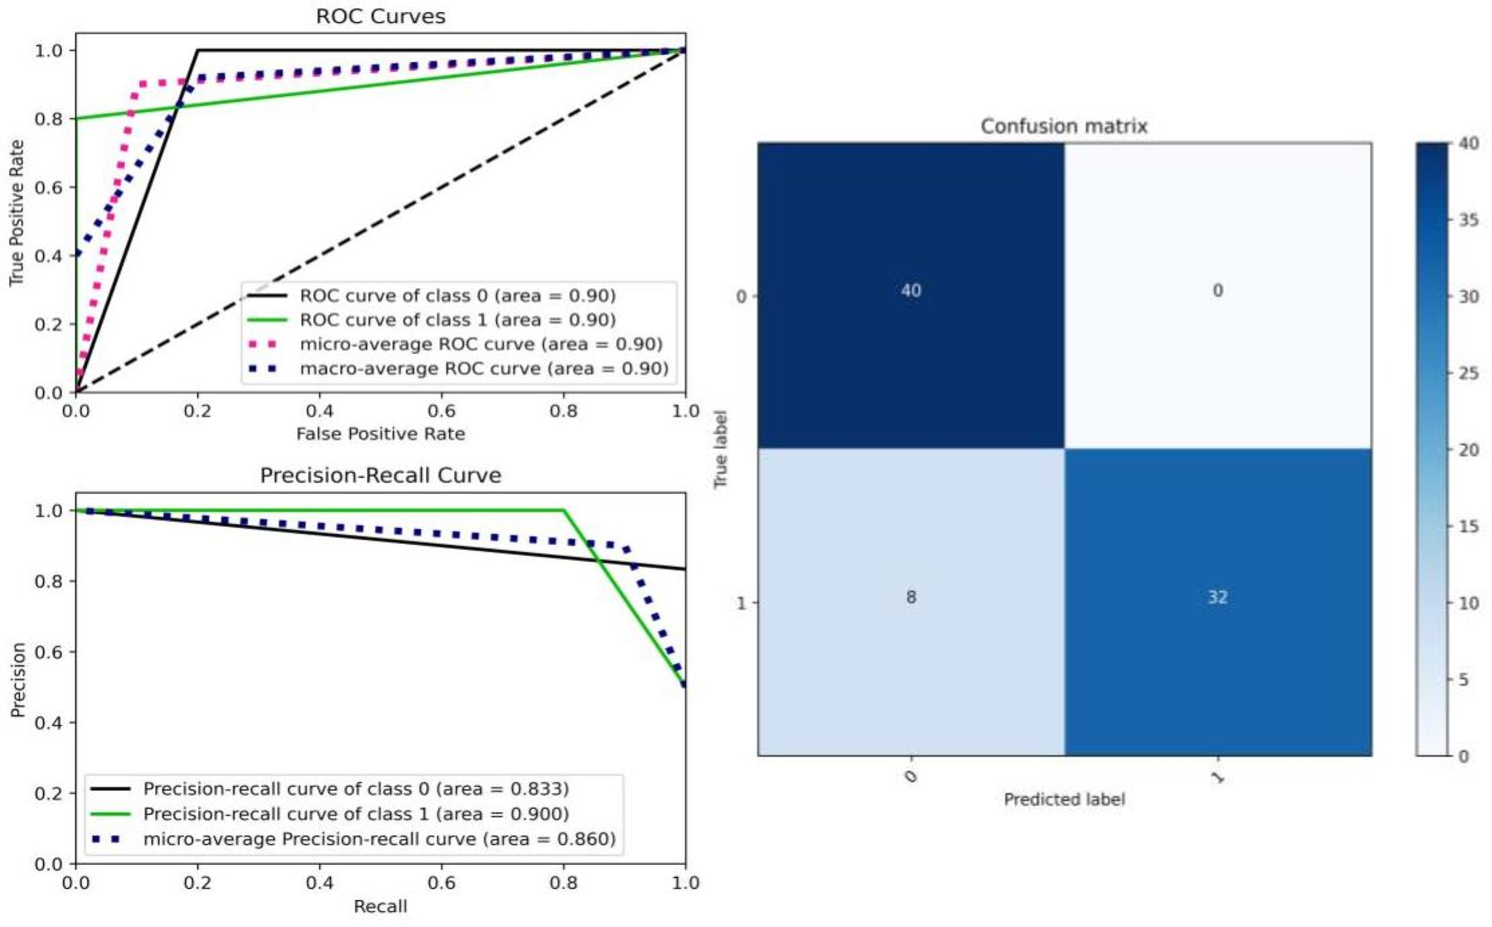
\includegraphics[width=\linewidth,keepaspectratio]{xzt.pdf}
    \caption{\texttt{x, z, time}: Classification Plots}
    \label{fig:xzt_results}
\end{figure}

\section{Dataset 3: \texttt{y, z, time}}
The \texttt{y, z, time} model reported 99\% accuracy score. The classification report in Table \ref{tab:yzt_classification_report} showed that the model did not incorrectly classify events as noise 98\% of the time. More importantly, it was able to correctly find and classify \textbf{all} event timeslices. 

\begin{table} [ht!]
    \centering
    \begin{tabular}{l c c c c}
    \hline
    \multicolumn{5}{c}{\texttt{y, z, time}} \\
    \hline
                     & precision & recall & F1-score & support \\
        \texttt{class\_0} & 1.00 &  0.97    & 0.99 & 40\\
        \texttt{class\_1} & 0.98 &  1.00    & 0.99 & 40\\
    \hline
    \end{tabular}
    \caption{\texttt{y, z, time}: Classification Report for \texttt{class\_0} and \texttt{class\_1}}
    \label{tab:yzt_classification_report}
\end{table}

Figure \ref{fig:yzt_results} shows the relevant plot of metrics for the dataset. The ROC and PR curves indicate very desirable results. The confusion matrix shows that out of the 40 test cases, all of the event timeslices were correctly labelled. Although one instance of noise timeslice was incorrectly classified as a timeslice with events. 

\begin{figure}[ht!]
    \centering
    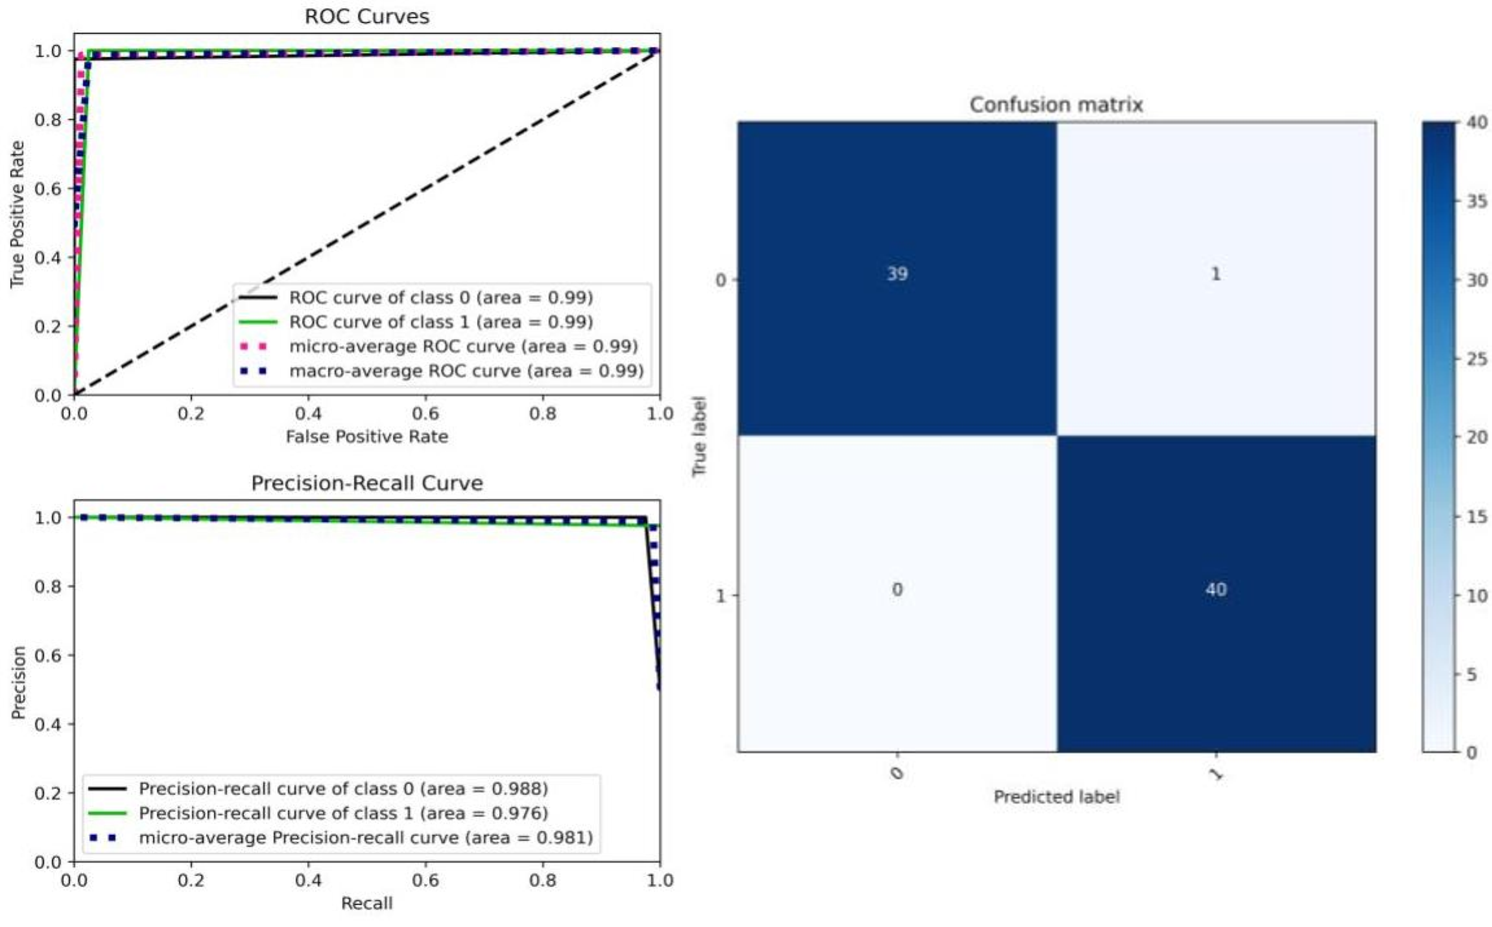
\includegraphics[width=\linewidth, keepaspectratio]{yzt.pdf}
    \caption{\texttt{y, z, time}: Classification Plots}
    \label{fig:yzt_results}
\end{figure}

Between the three datasets, the \texttt{y, z, time} model performed better than the other two, in terms of recall. It also had the highest F1 score for the positive class. The  \texttt{x, z, time} model performed poorly by wrongly classifying the most number of event timeslices. 


\section{Majority Voting Ensemble}
Next, results from the three models were combined using hard and soft voting. The classification reports in Tables \ref{tab:hard_classification_report} and  \ref{tab:soft_classification_report} show high precision, recall and F1 scores for hard voting. Soft voting on the other hand predicted much lower scores. It scored especially low on recall for \texttt{class\_1}.  The supporting plots in Figure \ref{fig:hard_plots} for hard majority voting corroborate to the precision and recall scores. Additionally, the final models were tested on the two edge cases - timeslices with very low event hits. All three models predicted both event timeslices to be noise timeslices. These results confirmed the visual inspection of the input meshes to PointNet (Section \ref{sec:eval_train_test_data}). Figure \ref{fig:soft_plots} shows the poorer performance of soft majority voting especially since 8 of the event timeslices were labelled as noise.

\begin{table} [ht!]
    \centering
    \begin{tabular}{l c c c c}
    \hline
    \multicolumn{5}{c}{Hard Voting: \texttt{(x y time), (x z time) (y z time)}} \\
    \hline
                          & precision & recall & f1-score & support \\
        \texttt{class\_0} & 0.95      &  1.00  & 0.98     & 40\\
        \texttt{class\_1} & 1.00 &    0.95     & 0.97     & 40\\
    \hline
    \end{tabular}
    \caption{Hard Voting: Classification Report for \texttt{class\_0} and \texttt{class\_1}}
    \label{tab:hard_classification_report}
\end{table}

\begin{table} [ht!]
    \centering
    \begin{tabular}{l c c c c}
    \hline
    \multicolumn{5}{c}{Soft Voting: \texttt{(x y time), (x z time) (y z time)}} \\
    \hline
                     & precision & recall & f1-score & support \\
        \texttt{class\_0} & 0.93 &  1.00    & 0.91 & 40\\
        \texttt{class\_1} & 1.00 &  0.80    & 0.89 & 40\\
    \hline
    \end{tabular}
    \caption{Soft Voting: Classification Report for \texttt{class\_0} and \texttt{class\_1}}
    \label{tab:soft_classification_report}
\end{table}


\begin{figure}[ht!]
    \centering
    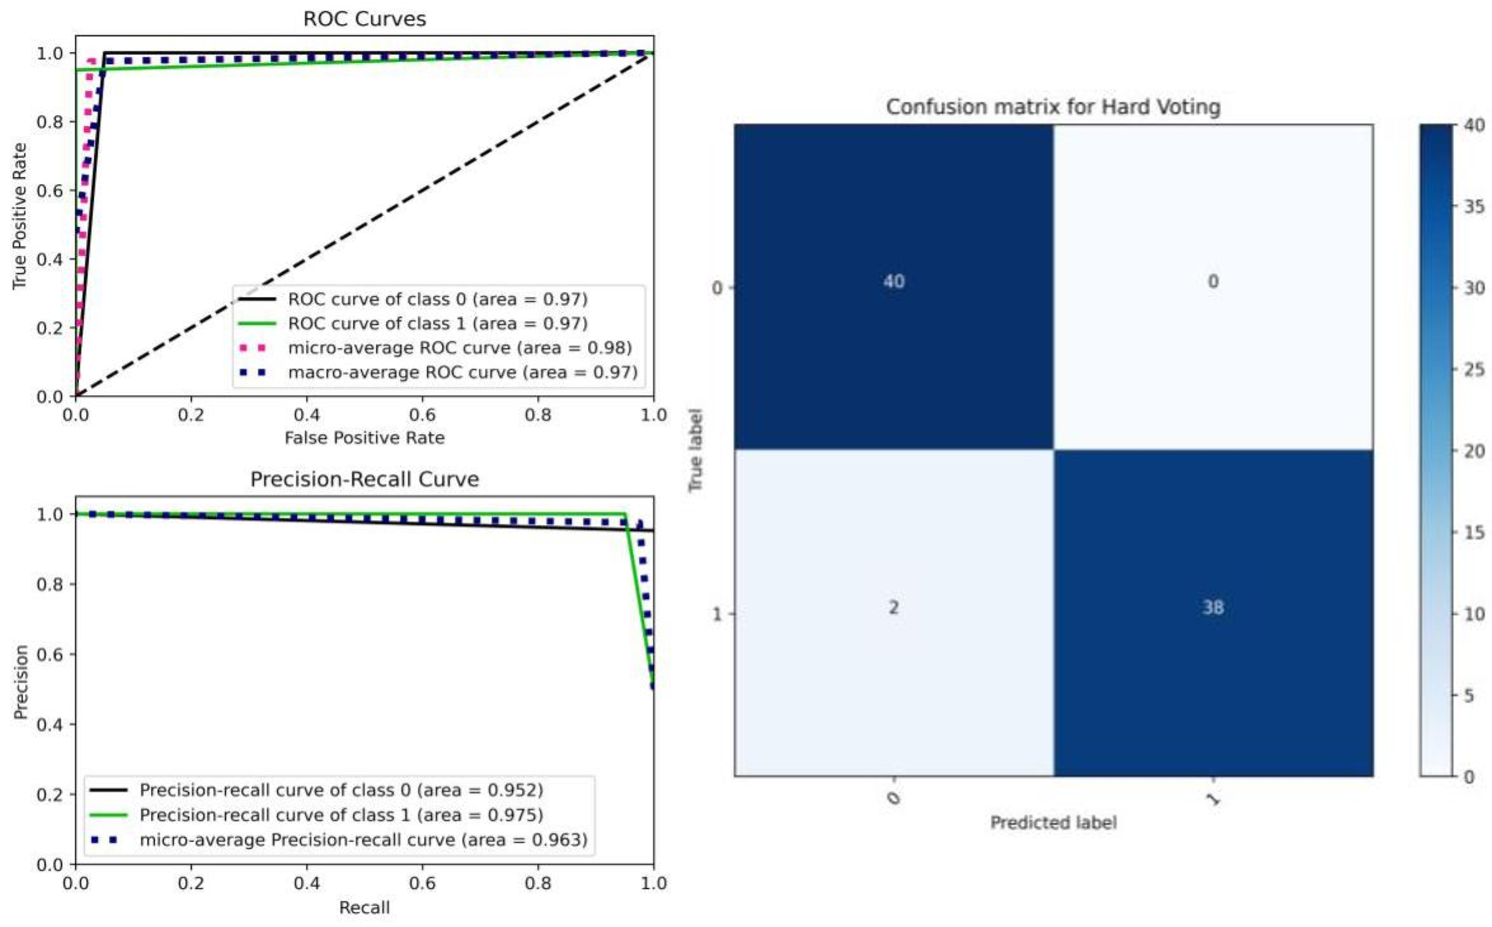
\includegraphics[width=0.9\linewidth, keepaspectratio]{hard_voting.pdf}
    \caption{Hard Voting Ensemble Results}
    \label{fig:hard_plots}
\end{figure}



\begin{figure}[ht!]
    \centering
    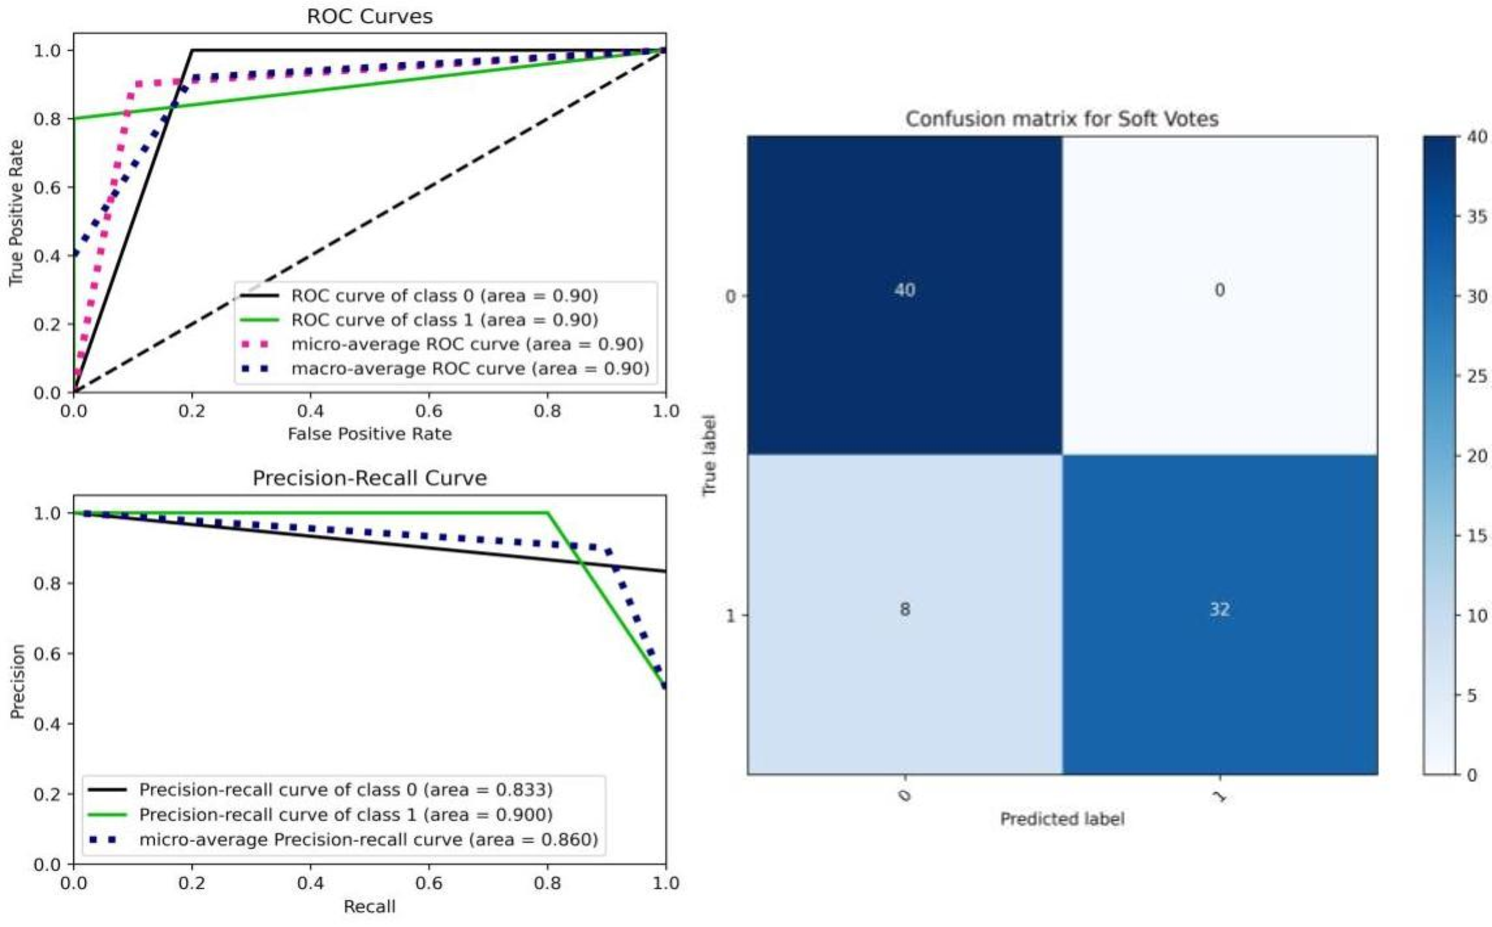
\includegraphics[width=0.95\linewidth, keepaspectratio]{soft_voting.pdf}
    \caption{Soft Voting Ensemble Results}
    \label{fig:soft_plots}
\end{figure}

\section{Comparison Against L1 Trigger}
The L1 trigger was applied to same test cases used for evaluating PointNet. Figure \ref{fig:l1} indicates that it can correctly classify all 40 event timeslices. However, it wrongly classified 5 noise timeslices. Like the PointNet model, it was unable to classify either of the two edge cases. Therefore, PointNet demonstrated better performance than L1 Trigger, especially in terms of minimising false positives. 

\begin{figure}[ht!]
    \centering
    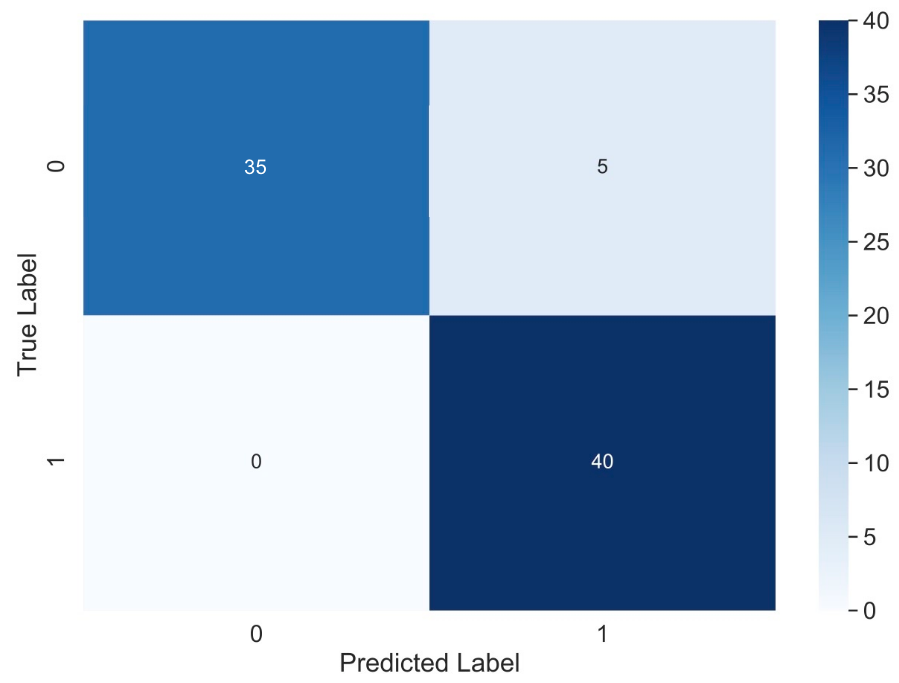
\includegraphics[width=\textwidth,height=5cm,keepaspectratio]{L1_results.png}
    \caption{Confusion Matrix From L1 Trigger to Testing Data}
    \label{fig:l1}
\end{figure}


\section{Other Performance Metrics}
Execution time for the pre-processing pipeline and the deep learning model was measured for the ensemble. Additionally, throughput and energy efficiency were calculated for the PointNet model. The ensemble comprised of the three datasets - (\texttt{x, y, time}), (\texttt{x, z, time}) and (\texttt{y, z, time}). Each dataset contained 400 timeslices, so a total of 1200 timeslices were processed. As each timeslice contained around 8000 rows, the complete ensemble had approximately 9,600,000 rows of data. The pre-processing was run on a Macbook Pro with 8GB of memory and 2 cores. All deep learning performance metrics were measured on Google Colab's Tesla T4 GPUs.

Python's \texttt{cProfile} \footnote{https://docs.python.org/3/library/profile.html} was used to obtain execution times for the complete pre-processing pipeline, starting from generation of 3D coordinates, to finally separating data into training and testing datasets. The total execution time was recorded to be \textit{3771.85 seconds} for the entire ensemble of three datasets. Figure \ref{fig:exec_time} shows the execution time for individual components of the pipeline. As expected, the main bottleneck arises from the conversion of 3D coordinates to 3D meshes. 

\begin{figure}[ht!]
    \centering
    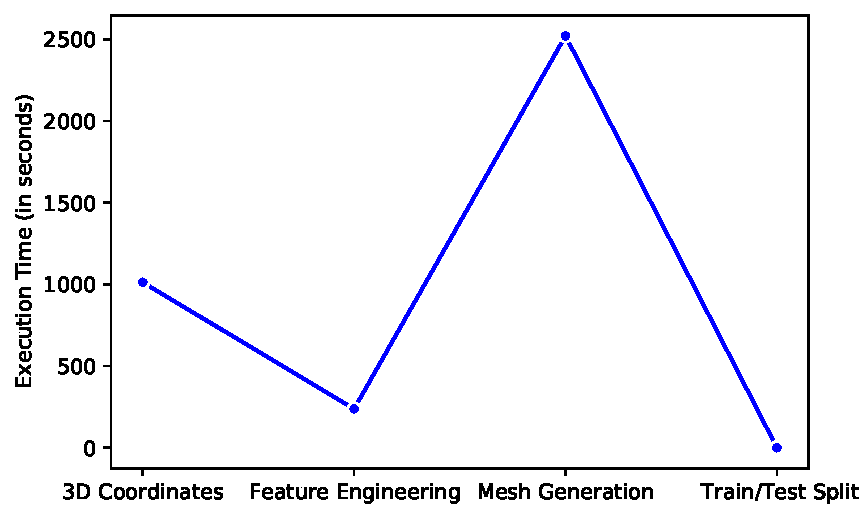
\includegraphics[width=0.8\textwidth,  height=5cm,keepaspectratio]{execution_time}
    \caption{Combined Execution Time for 3 Data sets for Each Stage in Pre-Processing Pipeline for the three datasets}
    \label{fig:exec_time}
\end{figure}

Next, execution time for PointNet was obtained, keeping in mind that execution time for deep learning typically involves only the feedforward functions \cite{yang2020note, teich2018plaster}. The three datasets were trained and evaluated in parallel, after which the results were combined. The mean execution time was measured to be \textit{94950.47 milliseconds (ms)} or \textit{1.5 minutes} and the total time for 120 epochs was approximately \textit{3.2 hours}.  

The throughput of a neural network can be stated as the maximum number of input the network can process in unit time and is an important metric for scalability \cite{hanhirova2018latency}.   The following formula was used to determine the throughput \cite{hanhirova2018latency}:

\begin{align*}
    \frac{(number \ of\ batches \times max\ batch\ size)}{(total\ time\ in\ seconds)}
\end{align*}

The maximum batch size for the GPU was found by performing a binary search and was \textit{64}. It was seen that the network could process \textit{0.34} input instances per second.

Finally, energy efficiency for the model was also calculated. Deep learning has the ability to solve complex tasks on specialised hardware, but are often energy intensive \cite{anthony2020carbontracker}. Energy metrics are not frequently reported in deep learning, but is significant in the present global climate \cite{anthony2020carbontracker}. Table \ref{tab:carbon}) shows the energy metrics for the PointNet model and was found using Python's \texttt{carbontracker}\footnote{https://pypi.org/project/carbontracker/}. The reported 62.4 g of CO2 emissions are relatively acceptable in comparison to an average of 4.5 kg CO2 emitted by standard deep learning models \cite{strubell2019energy}. 

\begin{table}[ht!]
    \centering
    \begin{tabular}{c l}
    \hline
    \multicolumn{2}{c}{Actual consumption for 1 epoch(s)} \\
    \hline
    Time & 0:01:38 \\
    Energy & 0.001770 kWh \\
    CO2eq & 0.520728 g \\
    \multicolumn{2}{c}{This is equivalent to:
	0.004325 km travelled by car} \\
	\hline
	\multicolumn{2}{c}{Predicted consumption for 120 epoch(s)}\\
	\hline
	Time & 3:16:20 \\
    Energy & 0.212393 kWh \\
    CO2eq & 62.487393 g \\
    \multicolumn{2}{c}{This is equivalent to:
	0.518998 km travelled by car} \\
	\hline
    \end{tabular}
    \caption{Energy Metrics and Carbon Footprint for PointNet}
    \label{tab:carbon}
\end{table}

The execution time for a single timeslice with 8500 hits including 700 event hits was also measured. The complete pipeline took 3.5 minutes from pre-processing and then obtaining a classification from the trained model. 


\section{Analysis}
Hard voting ensemble was chosen as the final result of PointNet classification project based on recall scores. Despite being considered naive, hard voting was suitable in this thesis since all three datasets more or less equally contributed to the learning. Since the three datasets are spatial combinations, none of them would have more valuable information about the neutrino events than the other. Soft voting resulted in lower performance as it was affected by the \texttt{x, z, time} recall scores. But since all three dataset models are equally important, a majority voting was more appropriate in finalising the results. 

Overall, the model was able to perform well in classifying timeslices into noise versus events. \textbf{97\%} of of the predictions were accurate overall. The final results showed that the model was able to correctly classify all noise timeslices and had a \textbf{95\%} recall for the positive class. All results showed that the models were better at classifying noise timeslices than event timeslices. This could be because of the feature engineering itself. As the network is tuned to handle class imbalances and overfitting, feature engineering could be insufficient in certain cases for timeslices with events. Out of 40, it only mis-classified 2 event timeslices as noise. While the recall for the positive class is not perfect, it met and exceeded the stakeholder requirement of 90\%. It also improved over the L1 trigger's performance in terms of identifying false positives. These scores have to be credited to the feature engineering and a high sampling of points per point cloud. Several experiments were conducted with the exact same network, but with no feature engineering. Here the model could not achieve more than 65\% accuracy in identifying positive classes (Appendix \ref{appendix-no-fe}). Additional experiments with the number of points sampled per point cloud showed that the higher the points sampled, the better. With the default 1024 points sampled and feature engineering, the model was able to perform only slightly better than before with 72\% accuracy. It was clear that due to the highly irregular shape of the mesh, with very low occurrences of significant areas, increasing the number of points sampled, increased the probability that points would be taken from the event cluster parts of the mesh. 

In terms of execution time, a single incoming timeslice will take 3.5 seconds to be classified. This is not ideal in real-time processing, where there may be incoming timeslices at every second. The proposed GPU pipeline in comparison is significantly faster \cite{karas_2019}.

This chapter examined results from the three datasets, focusing on the recall for positive class (\texttt{class\_1}). Results from the three datasets were combined using two majority voting techniques - hard and soft voting. Hard voting was chosen as the preferred, final result based on the best recall and precision scores. The results also showed improvements over the L1 trigger. There are no other similar approaches that can allow the project to make performance comparisons against, but the results can serve as a benchmark for future improvements. Additional execution, throughput and energy metrics also cannot be directly compared with other models. Instead, they can be used by KM3NeT to evaluate the feasibility of the model given their resources. 

\let\cleardoublepage\clearpage